%%%%%%%%%%%%%%%%%%%%%%%%%%%%%%%%%%%%%%%%%%%%%%%%%%%%%%%%%%%%%%%%%%%%%%%%%%%
%%%                                                                     %%%
%%%   LaTeX template voor het verslag van P&O: Computerwetenschappen.   %%%
%%%                                                                     %%%
%%%   Opties:                                                           %%%
%%%     tt1     Tussentijdsverslag 1                                    %%%
%%%     tt2     Tussentijdsverslag 2                                    %%%
%%%     tt3     Tussentijdsverslag 3                                    %%%
%%%     eind    Eindverslag                                             %%%
%%%                                                                     %%%
%%%   2 oktober 2012                                                    %%%
%%%   Versie 1.0                                                        %%%
%%%                                                                     %%%
%%%%%%%%%%%%%%%%%%%%%%%%%%%%%%%%%%%%%%%%%%%%%%%%%%%%%%%%%%%%%%%%%%%%%%%%%%%

\documentclass[tt3]{penoverslag}

%%% PACKAGES
\usepackage{lipsum}
\usepackage{gensymb}
\usepackage [dutch] {babel}
\usepackage{graphicx}
\usepackage{amsmath}
\usepackage{listings}
\usepackage{subcaption}
\usepackage{pgf,pgfplots}

\usetikzlibrary{fit,calc}
\usepgfplotslibrary{external}

\newcommand{\boxplot}[6]{%
	%#1: center, #2: median, #3: 1/4 quartile, #4: 3/4 quartile, #5: min, #6: max
	\filldraw[fill=white,line width=0.2mm] let \n{boxxl}={#1-0.1}, \n{boxxr}={#1+0.1} in (axis cs:\n{boxxl},#3) rectangle (axis cs:\n{boxxr},#4);   % draw the box
	\draw[line width=0.2mm, color=red] let \n{boxxl}={#1-0.1}, \n{boxxr}={#1+0.1} in (axis cs:\n{boxxl},#2) -- (axis cs:\n{boxxr},#2);             % median
	\draw[line width=0.2mm] (axis cs:#1,#4) -- (axis cs:#1,#6);                                                                           % bar up
	\draw[line width=0.2mm] let \n{whiskerl}={#1-0.025}, \n{whiskerr}={#1+0.025} in (axis cs:\n{whiskerl},#6) -- (axis cs:\n{whiskerr},#6);        % upper quartile
	\draw[line width=0.2mm] (axis cs:#1,#3) -- (axis cs:#1,#5);                                                                           % bar down
	\draw[line width=0.2mm] let \n{whiskerl}={#1-0.025}, \n{whiskerr}={#1+0.025} in (axis cs:\n{whiskerl},#5) -- (axis cs:\n{whiskerr},#5);        % lower quartile
	}

\begin{document}

% == VOORPAGINA == %
\team{Zilver} % teamkleur
\members{Sam Gielis\\
         Sophie Marien\\
         Toon Nolten\\
         Nele Rober\\
         Gerlinde Van Roey\\
         Maxim Van Mechelen} % teamleden

\maketitlepage

% == ABSTRACT EN INHOUDSTAFEL == %
\begin{abstract}
<<<<<<< HEAD
\label{ssec:abstr} % 3 ok
=======
\label{ssec:abstr} % 3 ?
>>>>>>> 012b513e084ceb15dd5546e6dd0b0183301679c4
Het P\&O-project bestaat erin een robot autonoom een doolhof te laten verkennen. Dit verslag beschrijft de invulling die team Zilver aan het project gaf. De robot wordt voorzien van een lichtsensor en een ultrasone sensor. Deze staan vast gemonteerd en kunnen niet onafhankelijk van de robot bewegen. De aansturing van de robot gebeurt via bluetoothverbinding. Een Grafische User Interface (GUI) maakt deze aansturing op een gebruiksvriendelijke manier mogelijk. De GUI geeft de baan van de robot  weer. Ook een historiek van de sensorwaarden wordt weergegeven in de GUI.

De robot kan zich autonoom door een doolhof voortbewegen zonder op muren te botsen. Tijdens het rijden slaat de robot een map op van de doolhof. Op elke nieuwe tegel kijkt de robot rond en geeft de gedetecteerde muren door. Wanneer de hele doolhof verkend is, gebruikt de robot het \textit{A*}-algoritme om de kortste weg naar de finish te bepalen. De finish wordt aangegeven met een bepaalde barcode. Andere barcodes laten de robot een opdracht uitvoeren.

Om de afwijking op de aansturing te minimaliseren, ori\"enteert de robot zich regelmatig op een witte lijn. Zo blijft de robot steeds zo dicht mogelijk bij het midden van de tegel.

Een computerprogramma simuleert de werking van de robot. Het is voor de simulator mogelijk door een virtuele doolhof te rijden en deze op gelijkaardige wijze te verkennen. De sensorwaarden worden gesimuleerd, met een afwijking om de werkelijke robot zo goed mogelijk te benaderen, maar verder worden dezelfde algoritmes gebruikt. Dit laat toe de algoritmes te testen zonder de robot hiervoor te gebruiken.

\end{abstract}

\tableofcontents

%figuur robot
\begin{figure}[!hb]
\begin{flushright}
    \includegraphics[width=1\textwidth]{robotFP2}
    \label{fig:robotFP}
\end{flushright}
\end{figure}


\newpage 

% == INLEIDING == %
\section{Inleiding} % 3 ok
\label{ssec:inl}
In het kader van het vak 'Probleemoplossen en Ontwerpen: computerwetenschappen' wordt gewerkt rond autonome intelligente robots. Verschillende teams bouwen en programmeren een robot met behulp van LEGO Mindstorms. Deze robot moet uiteindelijk volledig autonoom een doolhof kunnen verkennen.\\
Op de derde demonstratie kan de robot alle taken van de vorige demonstratie nog steeds uitvoeren. De robot kan zich volledig autonoom door een doolhof voortbewegen en hij kan deze in kaart brengen. Bij het inlezen van barcodes voert de robot een bepaalde opdracht uit. Op het moment dat de volledige doolhof is ingelezen, bepaalt de robot de kortste weg naar de barcode met code 'finish' en rijdt hier in hoge snelheid heen.

% == BOUW == %
\section{Bouw van de robot} % 3 ?
\label{sec:bouw}
LEGO Mindstorms\^{1} biedt een bouwpakket voor een robot aan. Een NXT-microcomputer laat toe de robot te programmeren met Java.

% == fysieke bouw == %
\subsection{Fysieke bouw} % 3 ?
\label{ssec:fysbouw}
Bij het bouwen van de robot (zie figuur \ref{robot}) werd het ontwerpboekje gevolgd dat bij het bouwpakket geleverd zat. Deze compacte samenstelling leek geen directe nadelen te hebben. Twee grote wielen worden elk met hun eigen motor aangestuurd. Kleine wielen achteraan zorgen voor meer stabiliteit en worden niet aangedreven. De sensoren werden als volgt ge\"implementeert: 

\begin{itemize}
\item \textit{lichtsensor:} vooraan en dicht tegen de grond.
\item \textit{ultrasone sensor:} bovenaan, naar voren kijkend. De sensor staat vast gemonteerd.
\item \textit{druksensoren:} aan beide zijkanten, \'e\'en aan de linkerkant en \'e\'en aan de rechterkant.
\end{itemize}

%figuur robot
\begin{figure}[tbp]
\begin{center}
    \includegraphics[width=0.8\textwidth]{robot}
    \caption{Robot}
    \label{robot}
\end{center}
\end{figure}


% figuur sensoren
\begin{figure}
        \centering
        \begin{subfigure}[h]{0.48\textwidth}
                \centering
                \includegraphics[width=\textwidth]{robotUS}
                \caption{Ultrasone sensor}
                \label{fig:US}
        \end{subfigure}%
        \begin{subfigure}[h]{0.48\textwidth}
                \centering
                \includegraphics[width=\textwidth]{robotLSTS}
                \caption{Licht- en Druksensor}
                \label{fig:LS+TS}
                \end{subfigure}
        \label{fig:sensors}
\end{figure}


Een alternatieve opstelling bestaat erin de NXT plat te leggen met ernaast de twee grote wielen. Op deze manier kan de ultrasone sensor op een extra motor gemonteerd worden zodat onafhankelijk van de robot kan ronddraaien. Deze opstelling vraagt echter om een nieuwe calibratie. Bovendien kan deze opstelling tot extra afrondingsfouten leiden. Omdat het voorlopig niet noodzakelijk is dat de ultrasone sensor kan ronddraaien, werd niet voor deze opstelling gekozen.


% == calibratie == %
\subsection{Calibratie van de motoren} % 3 MEETWAARDEN + BOXPLOT
\label{ssec:calibM}
De robot wordt aangedreven door twee motoren, elk verbonden met \'e\'en van de twee wielen. De aansturing gebeurt door te bepalen hoeveel graden de wielen moeten draaien. Beide wielen kunnen onafhankelijk ingesteld worden. De robot kan \'e\'en cm vooruit bewegen (beide wielen draaien x aantal graden in dezelfde richting) en rond zijn as (beide wielen draaien y aantal graden in tegengestelde richting). De resultaten van de calibratie worden weergegeven in tabel \ref{tab:resultCalibM}. Het bepalen van parameters x en y gebeurt als volgt:

%resultaten meetwaarden
\begin{table}[hb]
\begin{center}
    \begin{tabular}{  l || c | c | c }
     & linkerwiel & rechterwiel & aantal graden \\ \hline \hline
    1 cm vooruit & voor & voor & 20,8\degree
    \\ \hline
    1 cm achteruit & achter & achter & 20,8\degree
    \\ \hline
    180\degree draaien linksom & achter & linker & 701\degree \\ \hline
    180\degree draaien rechtsom & voor & achter & 701\degree \\
    \end{tabular}
    \caption{Resultaten calibratie motoren}
    \label{tab:resultCalibM}
\end{center}
\end{table}



\subsubsection{E\'en cm vooruit bewegen: bepalen van x} % 3 GEEN MEETWAARDEN VAN HET AANPASPROCES + BOXPLOT
\label{ssec:calibMx}
Een schatting voor x via de diameter van het wiel, waarbij x voor het aantal graden staat en de diameter in centimeter:

\begin{equation*}
x_{0} \approx \frac{360}{\pi \cdot diameter}
\end{equation*}

De parameter x kan verder bepaald worden via tests.
De robot rijdt naast een lintmeter tien keer tien cm af. De wielen draaien met andere woorden tien keer $10 \cdot x$ graden. De totale afwijking (in centimeter) op deze volledige meter is de som van alle afwijkingen op tien centimeter. Wanneer in \'e\'en keer \'e\'en meter wordt gereden is de totale afwijking kleiner.\\
Uit de test blijkt dat de robot een afwijking naar links heeft bij het rechtdoor rijden.

%boxplot motoren
\begin{figure}[tbp]
\begin{center}
    \includegraphics[width=0.8\textwidth]{boxplotLichtSensor}
    \caption{Boxplot meetwaarden motoren}
    \label{fig:boxMot}
\end{center}
\end{figure}

\subsubsection{Volledig rond de as draaien: bepalen van y} % 3 GEEN MEETWAARDEN VAN HET AANPASPROCES + BOXPLOT
\label{ssec:calibMy}

Een schatting voor y via de diameter van het wiel, met y in aantal graden en de as (afstand tussen beide wielen) en de diameter in centimeter:

\begin{equation*}
y_{0} \approx \frac{(2 \cdot \pi) \cdot (as_{robot}/2)}{diameter_{wiel}/2}
\end{equation*}

Om de robot om zijn as te laten draaien, bewegen de beide wielen in tegengestelde richting. De robot wordt naast een lijn geplaatst. De parameter wordt aangepast tot de robot na het draaien opnieuw precies naast de lijn uitkomt.

\subsection{Calibratie van de lichtsensor} % 3 BOXPLOT UPDATEN
\label{ssec:calibLS}
De lichtsensor meet de lichtintensiteit van de omgeving. De sensor kan zelf ook een rood licht uitsturen. Hoe meer dit licht geabsorbeerd wordt door de omgeving, hoe donkerder de omgeving. Op deze manier kunnen de meetwaarden ge\"interpreteerd worden als witte of zwarte lijnen.\\
De lichtsensor wordt in verschillende omstandigheden getest: bij direct kunstlicht (VL - veel licht), in de schaduw (WL - weinig licht), terwijl de robot rijdt (R - rijdend) en terwijl hij stilstaat (NR - niet rijdend). Dit voor alle soorten ondergrond: een paneel, een witte lijn of een zwarte lijn. De resultaten van deze metingen laten toe de lichtsensorwaarden de interpreteren en te simuleren. Een boxplot wordt weergegeven in figuur \ref{fig:boxLicht}. Deze toont dat het gemiddelde weinig afhangt van de omstandigheden. De afwijking wordt echter sterk bepaald door het feit of de robot rijdt of stilstaat.

\tikzset{external/remake next}
\begin{center}
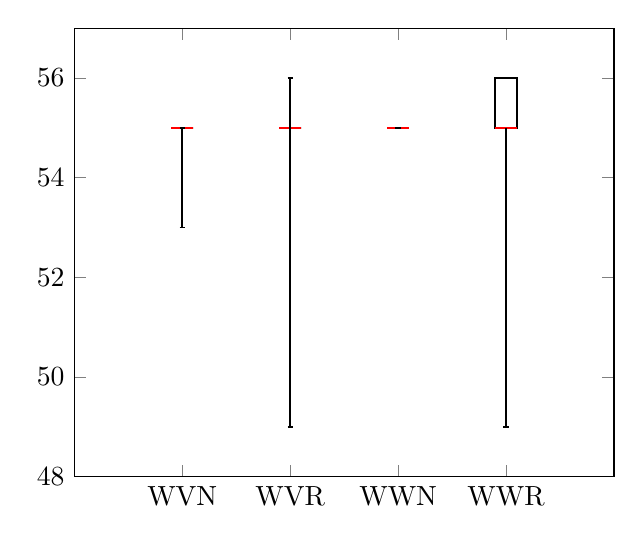
\begin{tikzpicture}
	\begin{axis}[xmin=0,xmax=5,ymin=48, ymax=57,
		xtick={1,2,3,4},xticklabels={WVN,WVR,WWN,WWR, PVN,PVR,PWN,PWR, ZVN,ZVR,ZWN,ZWR}]
		%#1: center, #2: median, #3: 1/4 quartile, #4: 3/4 quartile, #5: min, #6: max
		\boxplot{1}{55}{55}{55}{53}{55}
		\boxplot{2}{55}{55}{55}{49}{56}
		\boxplot{3}{55}{55}{55}{55}{55}
		\boxplot{4}{55}{55}{56}{49}{56}
	\end{axis}
    \label{box:boxLicht}
\end{tikzpicture}
\end{center}

\tikzset{external/remake next}
\begin{center}
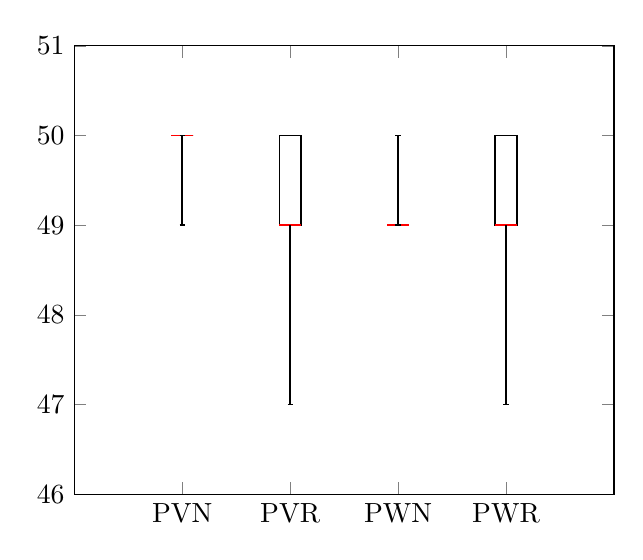
\begin{tikzpicture}
	\begin{axis}[xmin=0,xmax=5,ymin=46, ymax=51,
		xtick={1,2,3,4},xticklabels={PVN,PVR,PWN,PWR}]
		%#1: center, #2: median, #3: 1/4 quartile, #4: 3/4 quartile, #5: min, #6: max
		\boxplot{1}{50}{50}{50}{49}{50}
		\boxplot{2}{49}{49}{50}{47}{50}
		\boxplot{3}{49}{49}{49}{49}{50}
		\boxplot{4}{49}{49}{50}{47}{50}
	\end{axis}
    \label{box:boxLicht}
\end{tikzpicture}
\end{center}

\tikzset{external/remake next}
\begin{center}
\begin{tikzpicture}
	\begin{axis}[xmin=0,xmax=5,ymin=31, ymax=35,
		xtick={1,2,3,4},xticklabels={ZVN,ZVR,ZWN,ZWR}]
		%#1: center, #2: median, #3: 1/4 quartile, #4: 3/4 quartile, #5: min, #6: max
		\boxplot{1}{33}{33}{33}{32}{34}
		\boxplot{2}{33}{33}{33}{32}{34}
		\boxplot{3}{34}{34}{34}{34}{34}
		\boxplot{4}{34}{34}{34}{34}{34}
	\end{axis}
    \label{box:boxLicht}
\end{tikzpicture}
\end{center}

\subsection{Calibratie van de ultrasone sensor} % 3 TE WEINIG TESTS + BOXPLOTS
\label{ssec:calibUS}
Een ultrasone sensor zendt ultrasone geluidsgolven uit. De golven weerkaatsen op een object dat zich binnen het bereik bevindt. Bij ontvangst van zijn eigen geluidsgolven, weet de robot dat er een object in de buurt is.\\

In het kader van een doolhof, kan een robot muren tegenkomen als objecten. Maar ook de paaltjes, die de muren omhoog houden, worden als object gedetecteerd. Om een onderscheid te maken tussen de paaltjes en de muren, is er een nieuwe controle ingevoerd ten opzichte van de vorige demo. Uit testen bleek dat de robot de paaltjes wel degelijk als muren beschouwde en dit in bijna alle gevallen zo was. Vooral als de robot niet volledig op het midden van de tegel stond. Nu is er ingesteld dat een muur die gedetecteerd wordt, de waarde 29 of kleiner heeft als afstand. Als de robot de waarde 30 of groter doorgestuurd krijgt van de ultrasone sensor dan hebben we te maken met een paaltje.
% WELKE TESTEN?? MEETRESULTATEN!!!
De afwijking van de ultrasone sensor wordt gemeten door de robot op 30 cm van een muur te zetten en de bekomen meetwaarden te interpreteren. De robot staat in eerste instantie loodrecht ten opzichte van de muur en vervolgens met een afwijking van 20\degree van deze loodrecht stand. Een boxplot van de meetwaarden wordt weergegeven in figuur \ref{fig:boxUltra}.
% OOK VOOR ANDERE AFSTANDEN METEN!!!

\tikzset{external/remake next}
\begin{center}
\begin{tikzpicture}
	\begin{axis}[xmin=0,xmax=7,ymin=10, ymax=155,
		xtick={1,2,3,4,5,6},xticklabels={12.5,20,30,40,60, eind}]
		%#1: center, #2: median, #3: 1/4 quartile, #4: 3/4 quartile, #5: min, #6: max
		\boxplot{1}{16}{16}{16}{16}{16}
		\boxplot{2}{20}{20}{20}{20}{20}
		\boxplot{3}{30}{30}{30}{30}{30}
		\boxplot{4}{41}{41}{41}{40}{41}
		\boxplot{5}{61}{61}{61}{61}{56}
		\boxplot{6}{149}{148}{149}{147}{149}
	\end{axis}
    \label{box:boxLicht}
\end{tikzpicture}
\end{center}

% == ALGORITMES == %
\section{Algoritmes} % 3 ?
\label{sec:algo}
Verschillende algoritmes zorgen ervoor dat de robot alle opdrachten kan uitvoeren.

% == veelhoek == %
\subsection{Het rijden van een veelhoek} % 3 ?
\label{ssec:algoVeelH}
De robot en de simulator kunnen beiden een veelhoek rijden. Het aantal hoeken en de lengte van de zijden kunnen via de GUI ingesteld worden. De robot en de simulator rijden een afstand, draaien een bepaald aantal graden rond hun as, rijden weer dezelfde afstand,... Tot de volledige veelhoek gereden is. 

\lstset{frame=single, language=Java, caption=Veelhoek algoritme (pseudocode),
    	label=code:algoVeelH, numbers=left, numberstyle=\footnotesize,
		basicstyle=\sffamily, numbersep=5pt}
\begin{lstlisting}
Angle = (360.0/amtOfAngles)*100
Voor i van 0 tot amtOfAngles
	Beweeg lengthInCM vooruit
	Draai angle
\end{lstlisting}


% == witte lijn == %
\subsection{Het rechtzetten op een witte lijn} % 3 ?
\label{ssec:algoWitteL}
Indien regelmatig gecorrigeerd wordt op de calibratieafwijkingen kan de impact ervan geminimaliseerd worden. Deze correctie gebeurt door de witte lijnen als referentie te nemen en hier loodrecht op te ori\"enteren.
Onderstaand algoritme kan gebruikt worden wanneer de robot vlakbij een witte lijn staat (wanneer hij volledig rond zijn as draait zou hij de witte lijn moeten passeren):

\lstset{frame=single, caption=Witte Lijn algoritme (pseudocode),
		label=code:algoWitteL, numbers=left, numberstyle=\footnotesize,
		basicstyle=\sffamily, numbersep=5pt}
\begin{lstlisting}
AngleTurned = 0

Draai naar rechts tot witte lijn.
Draai naar links tot witte lijn EN verhoog AngleTurned.
Draai AngleTurned/2 naar rechts.
\end{lstlisting}

% IETS OVER TESTRESULTATEN + NAUWKEURIGHEID

Alternatief is het mogelijk te corrigeren op de muren, maar dan moet de robot zicht bevinden op een tegel die muren aan beide kanten bevat.


% == kortste pad == %
\subsection{Het vinden van het kortste pad} % 3 ?
\label{ssec:algoKortsteP}
Alvorens de robot het kortste pad tussen twee punten bepaalt, dient het hele doolhof gekend te zijn. Dit verkennen doet de robot autonoom. Elke tegel die de robot reeds passeerde, wordt gemarkeerd. Indien alle tegels gemarkeerd zijn, is de volledige doolhof doorzocht.
% HOE GEMARKEERD? MSS BETER EEN LIJST VAN NOG NIET BEKEKEN TEGELS?
Bij elke tegel onthoudt de robot alle uitwegen. Vervolgens slaat hij de eerste nog-niet-bekeken uitweg in. Wanneer de robot op een doodlopend stuk komt, keert hij terug tot een kruispunt waar nog niet alle uitwegen van bekeken werden.
Nadat de robot het hele doolhof bekeken heeft, kijkt hij na of de doolhof de 'finish'-barcode bevat. Indien niet, wordt het hele doolhof opnieuw onderzocht.
% NOG NIET GENOEG UITLEG OVER HET ALGORITME ZELF

Het kortste pad algoritme maakt gebruik van een graf die opgesteld wordt tijdens het verkennen van de doolhof. Het algoritme gebruikt de Manhattanafstand als heuristiek en de afgelegde afstand als kost.

% == SOFTWARE == %
\section{Software} % 3 ?
\label{sec:softw}
De software bestaat uit twee delen: een project dat op de NXT van de robot loopt en een project dat op de computer loopt. Alles wordt aangestuurd via de Graphical User Interface (GUI). Deze toepassing laat toe de robot te besturen (via bluetooth) en de reacties van de robot te simuleren met de simulator. Een Communication-pakket stuurt de commando's van de GUI door naar de juiste unit.
De simulator kan gebruikt worden om de software op te testen zonder telkens op de robot te moeten wachten.

% == software design == %
\subsection{Software ontwerp} % 3 ?
\label{ssec:Sdesign}
Zoals reeds vermeld bestaat de software uit twee projecten: \'e\'en draait op een computer en \'e\'en draait op de NXT-Brick. Figuren 4 en 5 tonen een klassendiagram.\\
Beide projecten hebben een identiek package \textit{commands} met \'e\'en klasse \textit{Command}. Hierin staan de final static integers die met de mogelijke bluetoothsignalen overeenkomen. Een verdere beschrijving van de software op de NXT-brick wordt in de sectie robot gegeven.\\
<<<<<<< HEAD
Het computerproject heeft nog 4 andere packages: \textit{communication}, \textit{gui}, \textit{simulator} en \textit{mapping}. 
=======


Het computerproject heeft nog zes andere packages: \textit{communication}, \textit{gui}, \textit{simulator}, \textit{mazeAlgorithm}, \textit{audio} en \textit{mapping}. 
>>>>>>> 012b513e084ceb15dd5546e6dd0b0183301679c4
De klasse \textit{SilverSurferGUI} uit de package \textit{gui} implementeert de GUI. De GUI communiceert met de simulator of de robot via de klassen in het package \textit{communication} door een object van de superklasse \textit{UnitCommunicator} bij te houden. Aan deze \textit{UnitCommunicator} is een object van de subklassen \textit{RobotCommunicator} of \textit{SimulatorCommunicator}  toegekend. Zo worden de commands dynamisch naar de juiste unit gestuurd: de \textit{RobotCommunicator} communiceert met het NXT-Project, de \textit{SimulatorCommunicator} met de simulator klassen.\\
Andere klassen van de package \textit{gui} zijn: \textit{MouseClickThread} , \textit{PolygonDrawThread}, \textit{RunForwardThread} en \textit{TurnAngleThread}. De vier Threads zorgen ervoor dat het tekenen van de baan van de robot de rest van het programma niet stillegt. \\
Het package \textit{simulator} implementeert de functionaliteit van de simulator. \\
Het \textit{mapping-package} heeft klassen zoals \textit{Tile, Edge, Obstruction, Barcode, ...} die elementen uit de wereld van een robot voorstellen. Een tile stemt overeen met \'e\'en tegel van het doolhof en heeft vier edges: \'e\'en voor elke zijde. Die edges houden de twee aanliggende tegels bij en eventueel een Obstruction, bijvoorbeeld een muur. De klasse \textit{MapGraph} brengt al deze elementen samen. Het houdt een begin-tegel bij en en huidige-tegel. Het biedt functionaliteiten aan om van de huidige tegel naar de tegel Noord, Oost, Zuid of West ervan te reizen en de map dynamisch uit te breiden. Zo wordt impliciet een hele graaf bijgehouden die dynamisch kan aangevuld worden. De klasse \textit{MapReader} kan uit een bepaalde textfile een MapGraph opstellen die overeenkomt met het doolhof dat in het bestand gedefinieerd wordt.


%figuur klassendiagram PC
\begin{figure}[tbp]
\begin{center}
    \includegraphics[width=0.8\textwidth]{KlassendiagramPC}
    \caption{Klassendiagram van de software die op de PC loopt}
    \label{fig:klasDiaPC}
\end{center}
\end{figure}

%figuur klassendiagram NXT
\begin{figure}[tbp]
\begin{center}
    \includegraphics[width=0.8\textwidth]{KlassendiagramNXT}
    \caption{Klassendiagram van de software die op de robot loopt}
	\label{fig:klasDiaNXT}
\end{center}
\end{figure}

% == commando's == %
\subsection{Het doorgeven van commando's} % 3 ok!
\label{ssec:commands}
De GUI zet een actie van de gebruiker om in een commando. Dit commando wordt gerepresenteerd door een integer dat naar de \textit{UnitCommunicator} wordt gestuurd. Twee van de commando's hebben echter extra informatie nodig: \textit{automatic move x cm forward} en \textit{rotate x degrees}. Deze informatie wordt toegevoegd aan de integer door de integer uit te breiden met extra cijfers (dit wordt in de volgende sectie in detail beschreven).\\
De \textit{UnitCommunicator} stuurt de bekomen integer door naar ofwel de \textit{RobotCommunicator} ofwel de \textit{SimulatorCommunicator}. Deze zetten de integer weer om in de juiste actie van respectievelijk de robot en de simulator. De wijze waarop dit gebeurt, verschilt licht voor beide gevallen. Zo stuurt de \textit{RobotCommunicator} zijn commando's via Bluetooth door naar de NXT-brick, terwijl de \textit{SimulatorCommunicator} zo'n verbinding niet nodig heeft.\\

\subsubsection{De bewerking op de integers} % 3 ok!
\label{sssec:integer}
Integers stellen de commando's voor. In twee gevallen is echter meer informatie nodig: om de robot een bepaalde afstand te laten afleggen en om de robot een bepaald aantal graden te laten draaien. Deze afstand en dit aantal graden moet mee doorgegeven worden met de integer. De eenheden waarin de afstand en de hoek worden doorgestuurd zijn respectievelijk cm en graden.\\\\
De doorgegeven integer wordt als volgt opgebouwd:

\begin{itemize}
\item de waarde van de afstand (hoek) wordt vermenigvuldigd met 1000.
\item de integer die het commando representeert, wordt hierbij opgeteld.
\end{itemize}

Om de bekomen resultaten terug op te splitsen in de twee oorspronkelijke gegevens worden volgende stappen gevolgd:

\begin{itemize}
\item een modulo-operatie van tien geeft het laatste cijfer terug. Dit stelt het soort commando voor.
\item dit getal wordt van de integer terug afgetrokken.
\item de oorspronkelijke afstand (hoek) wordt bekomen door de integer door 1000 te delen.
\end{itemize}

Deze werkwijze brengt een beperking met zich mee: de waarde van de afstand (hoek) kan slechts tot 2 cijfer(s) na de komma doorgegeven worden. De robot kan niet nauwkeuriger dan 0,1 cm aangestuurd worden. Hierdoor is het niet nodig de afstand nauwkeuriger door te geven. De nauwkeurigheid van de hoek is gevoeliger. De veelhoek stapelt immers veel afrondingsfouten op naarmate de lengte van de zijde en/of het aantal hoeken stijgt. Doordat de begin- en eindpunten niet samen vallen is te zien dat de som van de berekende hoeken samen geen 360 graden vormt. 

% == gui == %
\subsection{GUI} % 3 ?
\label{ssec:GUI}
De GUI bestaat uit twee vensters, enkele knoppen, een menubar en enkele instelmogelijkheden: zie figuur \ref{fig:gui}. Deze knoppen besturen ofwel de robot en de simulator ofwel enkel de simulator, naargelang de bluetooth verbinding aan staat. In deze sectie wordt verder enkel de robot vermeld. Dezelfde functionaliteiten gelden echter ook voor de simulator.

%overzicht functionaliteiten
\begin{itemize}
\item \textit{onderste venster:} debuginformatie van de robot.
\item \textit{bovenste venster:} tekent de baan van de robot. In latere demo's geeft dit venster ook de doolhof weer.
\item \textit{bluetooth connectieknop:} zet de verbinding aan of uit. Het icoontje ernaast verandert naargelang de status van de verbinding.
\item \textit{veelhoekinstellingen:} stellen de parameters van de veelhoek in. De 'Execute'-knop doet de robot een veelhoek rijden.
\item \textit{pijltjestoetsen:} besturen de robot manueel.
\item \textit{snelheidsinstellingen:} hiermee kan de snelheid van de robot aangepast worden.
\item \textit{clearknop:} wist de baan van de robot.
\item \textit{moveknop:} rij een bepaalde afstand vooruit of achteruit.
\item \textit{turnknop:} draai 90 graden naar rechts.
\item \textit{menubar:} submenu 'File' biedt de mogelijkheid om een doolhof-bestand te selecteren en in te lezen. Submenu 'Bluetooth' heeft dezelfde functionaliteit als de bluetooth-knop.
\end{itemize}

Twee parameters bepalen de veelhoek die de robot rijdt: het aantal hoeken van de figuur en de lengte van de zijden.
Een JSlider laat toe het aantal hoeken in te geven. Dit geeft de mogelijkheden overzichtelijk weer. Bovendien kan zo het bereik beperkt worden tot 30. Bij een groter aantal hoeken, streeft een veelhoek immers naar een cirkel.
Het bereik van de lengte van de zijden is groter: van \'e\'en centimeter tot een onbeperkte grootte. Hierdoor is het een betere optie om voor JSpinner te kiezen. Met de clearknop kan men het venster weer leeg maken. Hierbij wordt de positie van de robot behouden.
Voor de moveknop is er een Jslider voorzien net zoals voor de polygonDraw. Hiermee kan de afstand ingesteld worden dat de robot naar achter of naar voor moet rijden.

%figuur gui
\begin{figure}[tbp]
\begin{center}
    \includegraphics[width=0.8\textwidth]{GUI}
    \caption{Grafische User Interface}
	\label{fig:gui}
\end{center}
\end{figure}

% == bluetooth == %
\subsection{Bluetooth} % 3 ok!
\label{ssec:bluetooth}
De communicatie tussen robot en computer gebeurt volledig via bluetooth. De GUI voorziet een knop om deze verbinding te maken en geeft de status van de verbinding weer. De GUI stuurt commando's door naar de robot via de klassen \textit{UnitCommunicator} en \textit{RobotCommunicator}.

De leJOS-API\^{2} voorziet de \textit{NXTConnector} klasse. De methode \textit{connectTo((String, String, int, int)} zet de bluetoothverbinding tussen computer en brick op. De belangrijkste argumenten hiervoor zijn de naam van de NXT-Brick en zijn DeviceUrl  - in het geval van de gebruikte NXT: 'Silver' en '00:16:53:0A:04:5A'.

% == robot == %
\subsection{Robot} % 3 ?
\label{ssec:robot}
Een \textit{Finite State Machine} geeft de robot een concreet uitvoeringsschema. Een object van de klasse \textit{CommandUnit} houdt een currentState bij - een object van de superklasse \textit{State}. Negen subklassen verzorgen het nodige onderscheid: \textit{Waiting}, \textit{DrivingBackward}, \textit{TurnLeft}, \textit{DrivingRightForward}, …  en \'e\'en speciale toestand: de klasse \textit{Automatic}. De \textit{CommandUnit} ontvangt commando's via bluetooth. De \textit{CommandUnit} wijzigt de currentState naar een nieuw object van een \textit{State}-subklasse. De constructoren van elke subklasse passen het gedrag van de motoren aan bij de overgang naar de bepaalde state.
Bijvoorbeeld: De robot staat stil en zijn currentState is \textit{Waiting}.
Als de gebruiker de robot voorwaarts wil laten gaan, drukt hij de up-toets in. De \textit{CommandUnit} wijzigt de currentState van de robot naar currentState.ForwardPressed(). Dit levert een currentState van het type \textit{DrivingForward} op. De robot beweegt voorwaarts.
Tot slot is er de klasse \textit{Automatic}. Deze heeft vier methoden: \textit{turnAngle(int)}, \textit{driveForward(int)}, \textit{forwardToWhiteLine(LightSensor)} en \textit{whiteLinePerpendicular(LightSensor)}. De \textit{CommandUnit} roept deze methoden op met argumenten die hij geparsed heeft uit de informatie van de ontvangen signalen, zoals beschreven in sectie \ref{ssec:commands}.

% == simulator == %
\subsection{Simulator} % 3 ?
\label{ssec:simulator}
De simulator bootst de werking van de robot virtueel na. Hij kan dezelfde commando's uitvoeren als de werkelijke robot. De GUI stuurt de simulator aan via de klassen \textit{UnitCommunicator} en \textit{SimulatorCommunicator}. Deze ontvangen de uit te voeren commando's, analyseren ze en sturen ze door naar de simulator.
\\
De simulator zelf bestaat uit zeven klassen:

% overzicht klassen simulator
\begin{itemize}
\item \textit{Wall:} tekent de muren van het doolhof.
\item \textit{State:} wordt gebruikt om te zeggen of iets horizontaal of verticaal moet staan.
\item \textit{SimulationSensorData}
\item \textit{SimulationPilot:} houdt de positie en de richting van de 'robot' bij.
\item \textit{SimulationPanel:} tekent de baan van de 'robot' in het tekenpaneel.
\item \textit{GridDrawer:} zet het grid op.
\item \textit{Triangle:} berekent de hoekpunten van de driehoek die de 'robot' voorstelt.
\item \textit{ExtMath:} doet enkele berekeningen.
\end{itemize}

Het opzetten van het tekenpaneel gebeurt in de klasse \textit{SilverSurferGUI}. De klasse \textit{GridDrawer} voegt hier een grid aan toe. De roosters hebben dezelfde afmetingen als de secties van de panelen. Zo kan een muur enkel op een lijn van het grid staan.
Wanneer de 'robot' een pad aflegt, tekent de simulator dit in het tekenpaneel als een rode lijn (herschaald: \'e\'en cm = \'e\'en pixel). De lijn  bestaat uit verschillende cirkels die elkaar gedeeltelijk overlappen. Het \textit{SimulationPanel} houdt alle bezochte co\"ordinaten bij. De klasse bevat een methode die deze cirkels \'e\'en na \'e\'en tekent. Dit zorgt ervoor dat de lijn continu bijgewerkt wordt. De huidige positie en de huidige orientatie van de 'robot' wordt bovenaan het simulatorpaneel in de GUI weergegeven.

% == BESLUIT == %
\section{Besluit} % 3 ?
\label{sec:besl}
De uiteindelijke fysieke bouw van de robot bestaat uit de NXT, de wielen met aandrijvingen, een ultrasone sensor, een lichtsensor en twee druksensoren.
De calibratie van de robot zorgt ervoor dat hij precies aangestuurd kan worden en dat de sensoren waarden teruggeven die overeenkomen met de werkelijkheid.
De GUI gebruikt een eenvoudige interface en bevat knoppen waarmee de robot handmatig bestuurd kan worden. Door het ingeven van parameters in de GUI kan de robot een willekeurige veelhoek rijden. De uitleeswaarden van de sensoren vertellen de gebruiker wat de robot 'ziet'. Op deze manier krijgt de gebruiker een idee over de doolhof waar de robot in rijdt. Bovendien kan de robot zich loodrecht ori\"enteren op een witte lijn. De simulator is ook verbonden aan de GUI. Deze voert dezelfde opdracht uit als de robot. Het is mogelijk een virtueel doolhof te laten en de simulator hier in te laten 'rijden'. De simulator is handig om testen op uit te voeren, zonder steeds op de robot te moeten wachten.


\newpage
\makeappendix


% == DEMO 1 == %
\section{Demo 1} % 3 ok
\label{Asec:demo1}
De robot wordt voor demo 1 nog niet voorzien van sensoren. De focus ligt vooral op de nauw-keurigheid van de besturing en op het implementeren van alle softwarecomponenten. Deze software bestaat uit twee projecten: een op de computer en een op de robot. De robot kan een willekeurige veelhoek rijden en een simulator bootst de werking van de robot na.

% == resulaten == %
\subsection{Resultaten} % 3 ok
\label{Assec:result1}
Bij het rijden van de veelhoek had de robot een kleine afwijking. De afwijking werd groter bij grotere veelhoeken en meerdere hoeken om wille van de geaggregeerde fout.

% == conclusies == %
\subsection{Conclusies} % 3 ok
\label{Assec:conc1}
Calibratie moet meer getest worden. De GUI kan gebruiksvriendelijker, ook moet het scherm van de simulator herschaald worden, zodat de lijn van simulator nog wordt weergegeven als de simulator van de robot uit het scherm gaat.

% == aanpassingen == %
\subsection{Oplijsting aanpassingen verslag} % 3 ok
\label{Assec:aanp1}
Volgende secties werden aangepast ten opzichte van de eerste demonstratie:

% overzicht aangepaste secties
\begin{itemize}
\item \textit{\ref{ssec:fysbouw} Fysieke bouw:} de sensoren werden toegevoegd.
\item \textit{\ref{ssec:calibM} Calibratie van de motoren:} opnieuw gedaan.
\item \textit{\ref{ssec:calibLS} Calibratie van de lichtsensor:} nieuwe sectie.
\item \textit{\ref{ssec:calibUS} Calibratie van de ultrasone sensor:} nieuwe sectie.
\item \textit{\ref{ssec:algoVeelH} Het rijden van een veelhoek:} nieuwe sectie.
\item \textit{\ref{ssec:algoWitteL} Het rechtzetten op een witte lijn:} nieuwe sectie.
\item \textit{\ref{ssec:Sdesign} Software ontwerp:} enkele nieuwe klassen en mapping-package.
\item \textit{\ref{ssec:GUI} GUI:} enkele nieuwe functionaliteiten.
\item \textit{\ref{ssec:simulator} Simulator:} grid en triangle, virtuele doolhof.
\end{itemize}

% == DEMO 2 == %
\section{Demo 2} % 3 ok
\label{Asec:demo2}
De sensoren worden voor demo 2 wel ge\"installeerd. Na calibratie kunnen ze informatie doorzenden naar de robot. Threads zorgen ervoor dat de robot tegelijkertijd sensorwaarden kan lezen doorsturen.

De meetwaarden worden in de GUI weergegeven zodat een gebruiker de robot kan besturen zonder deze te zien. Bovendien is de simulator gekoppeld aan de robot. Wat de robot doet, doet de simulator ook en wordt getekend in de GUI. De simulator kan ook onafhankelijk van de robot opereren. Het is mogelijk een virtuele doolhof te laden en te simuleren dat de 'robot' zich hierdoor beweegt. Zowel robot als simulator kunnen zich rechtzetten op een (virtuele) witte lijn. Het is bovendien mogelijk de robot zich in het midden van de tegel te laten zetten.

% == resulaten == %
\subsection{Resultaten} % 3 ok
\label{Assec:result2}
Het verslag voor de tweede demonstratie bevatte enkele paragrafen die tegen het einde nog snel geschreven waren. Deze paragrafen waren van mindere kwaliteit. Ook sommige afbeeldingen werden verkeerd ingevoegd.

Op de demonstratie reed de robot de eerste tegels zoals het hoorde. Ook het witte lijnalgoritme werd goed uitgevoerd. De sensorwaarden werden weergegeven in de GUI, zodat de bestuurder, die de robot en het doolhof niet zag, zich een beeld kon vormen van het doolhof. Op een gegeven moment gaf de bestuurder de robot opdracht zich midden op een tegel te zetten. Dit algoritme maakt gebruik van de muren rond de tegel. De robot bevond zich op dat ogenblik echter op een tegel die door geen enkele muur omsloten werd. De bestuurder had dit niet eerst nagekeken. Dit had als gevolg dat de robot helemaal scheef stond, zonder dat de bestuurder dit wist.

De sensorwaarden werden niet gesimuleerd in de simulator. De simulator maakte in zijn algoritmes rechtstreeks gebruik van de virtuele doolhof. Robot en simulator maakten met andere woorden gebruik van andere algoritmes, wat niet het doel is van een simulator.

De simulator kon wel door een virtuele doolhof manoeuvreren. Meestal 'botste' hij tegen de muren, maar soms reed hij toch door een muur.

% == conclusies == %
\subsection{Conclusies} % 3 ok
\label{Assec:conc2}
Aan het verslag zou vroeger begonnen moeten worden zodat domme fouten vermeden kunnen worden.

De allign-algoritmes (op een witte lijn en in het midden van een tegel) werken enkel in specifieke situaties. De algoritmes dienen enkel in deze omstandigheden uitgevoerd te worden.

De simulator dient de sensorwaarden te simuleren en zou dezelfde algoritmes moeten gebruiken als de robot. Op deze manier kunnen de algoritmes getest worden zonder steeds op de robot te wachten.

% == aanpassingen == %
\subsection{Oplijsting aanpassingen verslag} % 3 ok
\label{Assec:aanp2}
Volgende secties werden aangepast ten opzichte van de tweede demonstratie:

% overzicht aangepaste secties
\begin{itemize}
\item \textit{\ref{ssec:abstr} Abstract:} aangepast.
\item \textit{\ref{ssec:calibLS} Calibratie van de lichtsensor:} meetresultaten toegevoegd.
\item \textit{\ref{ssec:calibUS} Calibratie van de ultrasone sensor:} meetresultaten toegevoegd en aangepast.
\item \textit{ Het rijden van een veelhoek:} er uitgehaald.
\item \textit{\ref{ssec:algoWitteL} Het rechtzetten op een witte lijn:} aangepast.
\item \textit{\ref{ssec:algoOnderzDoolhof} Algoritme onderzoeken doolhof:} nieuwe sectie.
\item \textit{\ref{ssec:AlgoKortsteP} Algoritme Kortste pad:} nieuwe sectie.
\item \textit{\ref{ssec:Sdesign} Software ontwerp:} enkele nieuwe klassen en packages.
\item \textit{\ref{ssec:GUI} GUI:} aangepast.
\item \textit{\ref{ssec:simulator} Simulator:} toevoegingen.
\end{itemize}

\newpage
\section*{Referenties}
\begin{enumerate}

\item \textit{Lego Mindstorms}:  Een uitbreiding op de LEGO bouwstenen waarmee kleine, aanpasbare en programmeerbare robots gebouwd kunnen worden. Een centrale besturingsmodule ('the brick') kan geprogrammeerd worden met verschillende programmeertalen. In eerdere versies werd een RCX gebruikt voor de brick, nu wordt met NXT gewerkt. De brick kan enkele motoren aandrijven. Bovendien kunnen er verschillende sensoren, o.a. een ultrasone sensor en een lichtsensor, aangesloten worden.  \mbox{[www.lego.com]} \mbox{[http://en.wikipedia.org/wiki/Lego\textendash Mindstorms]}

\item \textit{leJOS}:  Een kleine Java Virtuele Machine die toelaat de NXT-brick te programmeren. leJOS voorziet verschillende klassen die o.a. de motoren aansturen en een bluetoothverbinding opzetten.  \mbox{[http://lejos.sourceforge.net/]}

\end{enumerate}

\end{document}

